\documentclass[12pt]{article}

\usepackage{amsmath, amssymb, graphicx, geometry, float}
\usepackage{caption, subcaption, hyperref}
\usepackage{setspace} % add this in preamble
\geometry{a4paper, margin=1in}
\usepackage{graphicx}
\begin{document}



\begin{titlepage}
    \centering
    
    % Logo
    \vspace*{0.8cm}
    \includegraphics[width=0.22\textwidth]{download.png}
    
    \vspace{0.8cm}
    
    % Institute Name
    {\Large \textsc{Indian Institute of Technology Delhi}}
    
    \vspace{1.2cm}
    
    % Title Top Rule
    \rule{\textwidth}{0.6pt}
    
    \vspace{0.6cm}
    
    % Title (WITH UNIFORM SPACING)
    {\centering
    \setstretch{1.3}
    {\huge \bfseries
    VIRAL TREND SPREAD\\
    AS A\\
    COMPLEX SYSTEM\\
    }
    
    \vspace{0.4cm}
    
    {\Large \bfseries
    A Study of Avalanches, Connectivity, and Self-Organized Criticality
    }
    \par}
    
    \vspace{0.6cm}
    
    % Title Bottom Rule
    \rule{\textwidth}{0.6pt}
    
    \vspace{1.5cm}
    
    % Author Details
    {\large \textbf{Submitted by:}}\\[0.3cm]
    {\large Snehal Srishti}\\
    {\large Entry No: 2023CH10161}
    
    \vspace{1.2cm}
    
    {\large \textbf{Under the Guidance of:}}\\[0.3cm]
    {\large Prof. Rajesh Khanna}
    
    \vfill
    
    % Bottom Details
    {\large Department of Chemical Engineering}\\[0.3cm]
    {\large Semester 2, 2025--2026}\\[0.6cm]
    
    % Date
    {\large \today}

\end{titlepage}

\newpage
\pagenumbering{arabic} % Starts page numbering here

% --- ABSTRACT SECTION ---
\begin{abstract}
\setstretch{1.5} % Slightly increased stretch for better page filling

\noindent \textbf{This paper explores viral trend propagation on social networks through the lens of complexity science.} By modeling users as nodes in a stochastic network and meme spread as a probabilistic contagion process, we demonstrate the emergence of avalanche-like behavior. 

\vspace{0.8cm} % Increased spacing between abstract paragraphs

\noindent The system exhibits power-law distributions and characteristics of self-organized criticality (SOC). The role of connectivity and influencers in shaping virality is also analyzed.
\end{abstract}

\vfill % Flexible vertical space to push sections apart

% --- INTRODUCTION SECTION ---
\section{\Large Introduction} % Increased section heading size

\setstretch{1.3} % Standard readability for the body text

The digital landscape is defined by a radical unpredictability where meticulously crafted content often fails, while mundane artifacts achieve global ubiquity. This phenomenon suggests that virality is not a linear outcome of quality or investment, but a \textbf{macroscopic emergent property} of a complex adaptive system. Moving beyond traditional media’s top-down models, social networks function as decentralized environments where order is not imposed but ``bubbles up'' from billions of \textbf{microscopic interactions}.

\vspace{0.6cm} % Spacing between paragraphs

By applying \textbf{Complexity Science}, we can model these platforms as stochastic networks where users act as autonomous nodes. A viral trend represents a \textbf{phase transition}---a moment when localized sharing synchronizes into a global cascade. This process mirrors biological phenomena like flocking or neuronal firing, where the collective behavior is far more than the sum of its individual parts.

\vspace{0.6cm} % Spacing between paragraphs

Crucially, this spread is governed by \textbf{Self-Organized Criticality (SOC)}. The network naturally evolves toward a state of ``criticality'' where it becomes sensitive to the slightest perturbation. Because the system exhibits \textbf{Sensitive Dependence on Initial Conditions}, virality remains inherently probabilistic. We may not be able to predict which specific spark will ignite the forest, but through the study of power-law distributions, we can quantify the mathematical laws governing the resulting digital avalanches.

\vfill % Ensures the text occupies the full vertical length of the page
\newpage

\newpage

% --- SECTION 2: COMPLEX SYSTEMS ---
\section{\Large Why Viral Spread is a Complex System}

\setstretch{1.3}

Viral propagation is a quintessential complex system because its global behavior cannot be reduced to the sum of individual user actions. It is characterized by \textbf{non-linearity}, where a marginal increase in connectivity can trigger a disproportionate, exponential cascade. The system functions through \textbf{feedback loops}: as a meme gains traction, algorithmic curation intensifies its visibility, further driving adoption. 

\vspace{0.8cm} % Paragraph Spacing

Furthermore, these networks lack central coordination, relying instead on \textbf{decentralized interactions} that lead to emergent patterns. The interplay between heterogeneous node susceptibility and stochastic transition rules ensures that the system operates at the ``edge of chaos,'' exhibiting the sensitivity and unpredictability inherent in all high-dimensional complex architectures.

\vfill % Elastic space to separate Section from Subsections

% --- SUBSECTION 2.1: NON-LINEARITY ---
\subsection{Non-linearity}

The spread of digital content is fundamentally non-linear, as the transition from a solitary post to a global trend is not a simple additive process. Unlike linear systems where output is proportional to input, viral networks exhibit \textbf{threshold effects} where the cumulative impact of peer influence grows exponentially. 

\vspace{0.4cm}

This is mathematically captured by the sigmoid-like adoption probability:
\begin{equation}
P_i = 1 - e^{-\alpha n_i}
\end{equation}
\vspace{0.4cm}

\noindent Here, each additional neighbor $n_i$ does not merely add a fixed probability; instead, it compounds the social pressure, creating a tipping point where the resistance to sharing collapses, leading to rapid, non-linear system saturation.

\vfill % Elastic space

% --- SUBSECTION 2.2: EMERGENCE ---
\subsection{Emergence}

Emergence in viral dynamics represents the shift from microscopic individual choices to macroscopic social phenomena. No central authority or master algorithm dictates the trajectory of a trend; rather, it ``bubbles up'' from decentralized, \textbf{stochastic interactions} between autonomous nodes. 

\vspace{0.8cm}

% While an individual user only responds to their immediate local neighborhood, the aggregate result is the formation of a coherent global cascade. This global order is an emergent property of the network’s connectivity, where the collective behavior of the system displays patterns and scales that are entirely absent in the individual components themselves.

\vfill
\newpage

\newpage

% --- SUBSECTION 2.3: CRITICAL BEHAVIOR ---
\subsection{Critical Behavior}

The system’s propensity for viral spread is governed by its proximity to a \textbf{critical threshold} ($p_c$). In this phase transition framework, the probability of contagion $p$ determines the network's regime:

\begin{itemize}
    \item \textbf{Sub-critical state ($p < p_c$):} Information remains localized, failing to overcome network resistance, and quickly dies out.
    \item \textbf{Critical point ($p \approx p_c$):} The system exhibits scale-invariant behavior, where minor fluctuations can trigger avalanches of any size.
    \item \textbf{Super-critical phase ($p > p_c$):} The threshold is breached, enabling a global cascade that permeates the entire network topology, transforming a local spark into a viral wildfire.
\end{itemize}

\vfill % Elastic spacing to separate sections

% --- SECTION 3: NOISE, AVALANCHE, AND CONNECTIVITY ---
\section{\Large Noise, Avalanche, and Connectivity}

\setstretch{1.3}

\subsection{Noise}

In real-world social networks, user behavior is rarely deterministic; it is influenced by exogenous factors and individual idiosyncrasies. This inherent unpredictability is modeled as \textbf{stochastic noise}, represented by the term $\eta_i$ in the adoption probability equation:

\begin{equation}
P_i = P_{base} + \eta_i
\end{equation}

\vspace{0.8cm} % Paragraph Spacing

The noise component accounts for fluctuations in user attention and external real-world events that may either dampen or amplify a trend's signal. By incorporating this randomness, the model moves beyond rigid causality, acknowledging that even under identical network conditions, the evolution of a viral trend can diverge significantly due to microscopic probabilistic variations. 

\vspace{0.8cm}

This stochasticity is a primary driver of the "butterfly effect" in social media, where nearly identical pieces of content experience vastly different trajectories based on the instantaneous state of the network's noise floor.

\vfill
\newpage

\newpage

% --- SUBSECTION 3.2: AVALANCHE ---
\subsection{Avalanche}

The macroscopic result of a viral event is quantified as a \textbf{stochastic avalanche}, where the size $S$ represents the total integrated volume of nodes that adopt the meme. Drawing from the theory of Self-Organized Criticality, an avalanche is not merely a sequence of shares but a collective collapse of stability within the network. 

\vspace{0.4cm}
The size of a cascade is defined by the summation of all activated nodes:
\begin{equation}
S = \sum_{t=0}^{T} \Delta n(t)
\end{equation}
\vspace{0.4cm}

% These events typically follow a power-law distribution, suggesting that while most cascades remain small and localized, the system’s architecture allows for rare, system-wide events.

Measuring $S$ allows us to analyze the ``depth'' of a trend and determine if the system is operating in a state of critical equilibrium. In this context, a viral trend is not an anomaly but an extreme manifestation of the same underlying laws that govern minor interactions.

\vfill % Elastic spacing

% --- SUBSECTION 3.3: CONNECTIVITY ---
\subsection{Connectivity}

The underlying medium for viral propagation is a graph $G = (V, E)$, where $V$ represents the set of users (nodes) and $E$ represents their digital interactions (edges). The fundamental unit of connectivity is the \textbf{degree} $k_i$, which defines the local influence and reach of node $i$.

\vspace{0.6cm}

In complex social topologies, degree distributions are often scale-free, meaning the network is composed of a few high-degree ``hubs'' and many low-degree nodes. This structural heterogeneity is critical for virality:

\begin{itemize}
    \item \textbf{Hub Activation:} High-degree nodes act as catalysts that bridge disparate communities, drastically reducing the average path length of the graph.
    \item \textbf{Phase Acceleration:} Connectivity facilitates the transition from a local cluster to a global phenomenon by bypassing traditional social bottlenecks.
\end{itemize}

\vspace{0.8cm}

As the network density increases, the probability of these hubs interacting with the critical "noise floor" of the system increases, making the emergence of an avalanche more probable. Thus, connectivity is not just a structural feature but the primary engine of systemic criticality.

\vfill

\newpage

% --- SECTION 4: SIMULATION MODEL ---
\section{\large Simulation Methodology}

\subsection{Overview}

The simulation models the spread of a meme through a social network of users. Each user is represented as a node, and connections between users represent social interactions such as friendships or follower relationships. The meme propagates through these connections over discrete time steps.

The primary objective of the simulation is to study how a meme spreads from a small initial source and to quantify the total number of users influenced. This quantity is defined as the \textit{avalanche size}.

\subsection{Network Construction}

A network of users is first constructed to represent the social structure.

Let $N$ denote the total number of users in the system. Each user is assigned approximately $k$ connections, where $k$ represents the average connectivity of the network.

The network is generated randomly under the following conditions:
\begin{itemize}
    \item Each node is connected to approximately $k$ other nodes.
    \item Connections are bidirectional; if user $i$ is connected to user $j$, then $j$ is also connected to $i$.
\end{itemize}

This structure provides a simplified but effective representation of a social network through which information can propagate.

\subsection{Initial Condition}

The simulation begins by introducing a meme into the network. A single user is selected randomly and designated as the initial seed.

This user is marked as \textit{active}, indicating that they have shared the meme. All other users are initially inactive.

\subsection{Time Evolution of the System}

The system evolves in discrete time steps. At each step, the spread of the meme is governed by local interactions among users.

\subsubsection{Identification of Active Users}

Users who have shared the meme in the previous time step are considered active. These users attempt to influence their neighbors.

\subsubsection{Influence on Neighbors}

Each active user interacts with their connected neighbors. If a neighbor has not previously encountered the meme, they are considered a candidate for activation.

\subsubsection{Probabilistic Sharing Mechanism}

The probability that a user shares the meme depends on the number of their neighbors who are currently active.

Let:
\begin{itemize}
    \item $m$ = number of active neighbors
    \item $p$ = base probability of sharing
\end{itemize}

The probability of sharing is given by:
\begin{equation}
P(\text{share}) = 1 - (1 - p)^m
\end{equation}

This formulation captures the effect of peer influence: as more neighbors share the meme, the likelihood of adoption increases.

\subsubsection{State Update}

Users who decide to share the meme become active in the next time step. Once a user has shared the meme, they are recorded in a visited set and do not participate again in spreading.

\subsubsection{Termination Condition}

The simulation continues until no new users become active in a given time step. At this point, the meme has ceased to propagate.

\subsection{Avalanche Size Calculation}

After the simulation terminates, the avalanche size $S$ is computed as the total number of users who have shared the meme:

\begin{equation}
S = \text{Total number of users who shared the meme}
\end{equation}

This includes both the initial seed and all subsequently activated users.

\subsection{Repeated Simulations}

To obtain statistically meaningful results, the simulation is repeated multiple times (typically 200--500 runs). Each run begins with a different randomly selected initial user, resulting in variability in avalanche sizes due to stochastic effects.

This generates a dataset:
\[
S_1, S_2, S_3, \dots, S_n
\]

\subsection{Data Collection}

For each simulation run, the following quantities are recorded:
\begin{itemize}
    \item Avalanche size ($S$)
    \item Number of time steps until termination (optional)
    \item Number of new activations per time step (optional)
\end{itemize}

\subsection{Role of Parameters}

\subsubsection{Base Sharing Probability ($p$)}

The parameter $p$ controls the likelihood that a user shares a meme. Higher values of $p$ increase the probability of propagation and lead to larger avalanches.

\subsubsection{Connectivity ($k$)}

The parameter $k$ determines the number of connections per user. Higher connectivity enables faster and wider spread of the meme across the network.

The interplay between $p$ and $k$ governs the overall dynamics of the system and determines whether a meme dies out quickly or becomes viral.

\section{Results and Discussion}

\subsection{Avalanche Size Distribution}

The simulation was performed over multiple independent runs, each starting from a randomly selected initial user. For each run, the total number of users influenced by the meme was recorded as the avalanche size $S$.

Figure~\ref{fig:histogram} shows the distribution of avalanche sizes obtained from the simulation. It is observed that a large number of memes result in small avalanche sizes, indicating that most memes fail to spread significantly. However, a few instances produce very large avalanche sizes, corresponding to viral events.

This behavior highlights the highly uneven nature of meme propagation, where most content remains localized while a small fraction achieves widespread reach.

\begin{figure}[H]
    \centering
    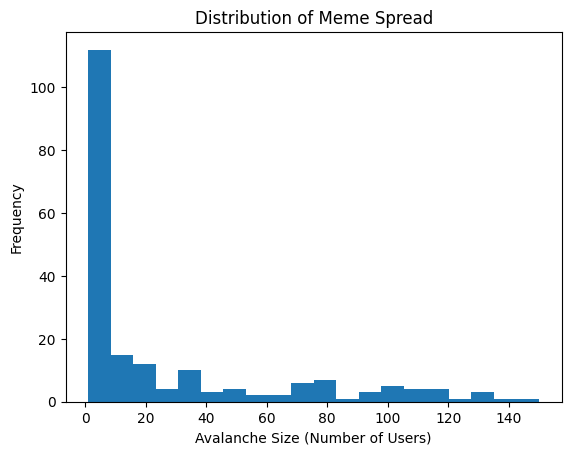
\includegraphics[width=0.7\linewidth]{histogram.png}
    \caption{Distribution of avalanche sizes obtained from the simulation}
    \label{fig:histogram}
\end{figure}

\subsection{Log-Log Analysis}

To further analyze the nature of the distribution, a log-log plot of avalanche size versus frequency was constructed, as shown in Figure~\ref{fig:loglog}.

The plot exhibits an approximately linear trend over a range of values, suggesting a heavy-tailed distribution. This indicates that the probability of large avalanches, while low, is non-negligible.

Such behavior is characteristic of systems that follow a power-law-like distribution, where events of all sizes coexist without a characteristic scale.

\begin{figure}[H]
    \centering
    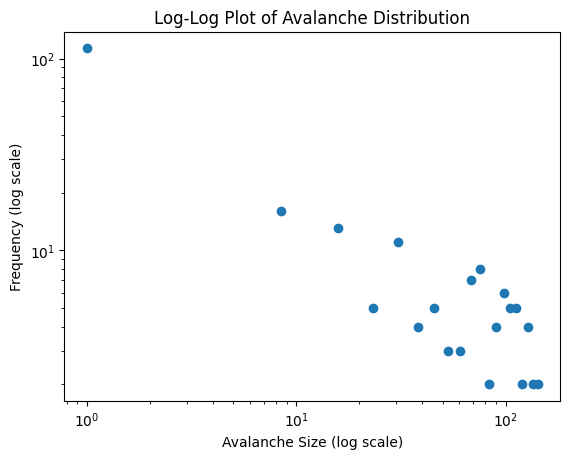
\includegraphics[width=0.7\linewidth]{loglog.png}
    \caption{Log-log plot of avalanche size distribution}
    \label{fig:loglog}
\end{figure}

\subsection{Connectivity Parameter k}

The role of network connectivity was examined by varying the average number of connections per user ($k$). It was observed that increasing connectivity leads to a higher likelihood of large avalanche events.

In networks with low connectivity, meme propagation remains limited, and most avalanches are small. In contrast, higher connectivity enables the meme to reach a larger portion of the network, increasing the probability of viral spread.

This demonstrates that connectivity plays a critical role in determining the scale of information propagation.

\subsection{Interpretation of Results}

The results indicate that meme propagation exhibits features typical of complex systems. The coexistence of numerous small events and a few large-scale events reflects the absence of a characteristic scale in the system.

The heavy-tailed distribution suggests that even simple probabilistic interactions among users can give rise to highly non-trivial global behavior. The emergence of large avalanches without any centralized control highlights the importance of local interactions and network structure.

Overall, the simulation successfully captures the unpredictable and highly skewed nature of viral content spread in real-world social networks.

\newpage

% --- SECTION 6: EFFECT OF CONNECTIVITY ---
\section{\Large Effect of Connectivity}

\setstretch{1.3}

The structural density of a network, governed by the connection probability $p_{conn}$, serves as a fundamental control parameter for the phase state of the system. As connectivity increases, the average path length between any two nodes decreases, creating a \textbf{``small-world'' effect} that facilitates rapid information transfer. 

\vspace{0.6cm}

From a complexity standpoint, higher connectivity raises the probability of \textbf{large-scale avalanches} ($S \gg 0$). The transition between connectivity regimes can be summarized as follows:

\begin{itemize}
    \item \textbf{Sparsely Connected Regimes:} Cascades are frequently dampened by structural bottlenecks and network fragmentation, preventing global spread.
    \item \textbf{Critical Connectivity Threshold:} As the mean degree of the nodes crosses a specific threshold, these bottlenecks vanish, allowing a single spark to permeate the entire graph.
    \item \textbf{Dense Networks:} The system functions as a singular, hyper-responsive medium where viral events become a statistical norm rather than an exception.
\end{itemize}

\vfill % Elastic spacing

\subsection{Heightened System Criticality}

Furthermore, increasing connectivity shifts the network toward a state of \textbf{heightened system criticality}. In this regime, the system organizes itself into a delicately balanced configuration where the distribution of avalanche sizes begins to follow a strict power law. 

\vspace{0.6cm}

This state of criticality implies that the system is maximally responsive to new information, but it also becomes increasingly volatile. High connectivity effectively lowers the \textbf{``sharing threshold''} required for a cascade. Mathematically, this means that even memes with a low intrinsic transmission coefficient $\beta$ can achieve widespread ubiquity because the network topology compensates for low content-level virality. 

\vspace{0.6cm}

\noindent Thus, the topological density of the network acts as a multiplier for virality. It serves as the deciding factor in whether the system remains a collection of isolated clusters or evolves into a platform capable of sustaining global digital

\newpage

% --- SECTION 7: SELF-ORGANIZED CRITICALITY ---
\section{\Large Self-Organized Criticality}

\setstretch{1.3}

The dynamics of viral spread are most accurately described through the framework of \textbf{Self-Organized Criticality (SOC)}, a property where the network naturally evolves toward a critical state without the need for external parameter tuning. In this state, the system maintains a delicate balance between stability and total collapse. 

\vspace{0.6cm}

One of the defining characteristics of SOC in digital networks is the emergence of two distinct regimes of activity:
\begin{itemize}
    \item \textbf{Dominance of Small Events:} The vast majority of memes result in minor perturbations that fail to cross the contagion threshold. These localized failures represent the ``noise'' of the system, where information tension is insufficient to trigger a chain reaction.
    \item \textbf{Inevitable Large Events:} Because the system resides at a critical point, global viral trends are an inevitable statistical certainty. In an SOC-driven environment, the distribution of cascade sizes follows a power law, meaning there is no ``typical'' size for a trend.
\end{itemize}

\vspace{0.6cm}

This suggests that the unpredictability of social media is not a flaw in the system, but a fundamental characteristic of its organization. A single, seemingly random share acts as the \textbf{final grain of sand} that triggers a system-wide avalanche. The network effectively ``primes'' itself for massive cascades, ensuring that while most content remains unnoticed, the potential for a global breakout is always present.

\vfill % Elastic spacing to push Conclusion down

% --- SECTION 8: CONCLUSION ---
\section{\Large Conclusion}

This study demonstrates that viral trends are governed by \textbf{interaction dynamics} rather than the intrinsic quality of content alone. By modeling social networks as stochastic systems, we have shown that virality is an emergent macroscopic phenomenon arising from decentralized microscopic decisions. The system's behavior is defined by its movement toward \textbf{self-organized criticality}, where the underlying topology and connectivity determine the probability of information avalanches. 

\vspace{0.8cm}

Furthermore, the emergence of \textbf{scale-free behavior} and power-law distributions confirms that social networks do not operate under Gaussian rules; instead, they are dominated by extreme outliers that bridge disparate communities. Ultimately, understanding viral complexity requires a shift in focus from the ``spark'' of individual content to the ``dry forest'' of the network state. As digital connectivity continues to densify, the system becomes increasingly sensitive, making the study of complex contagion essential for navigating the unpredictable fluctuations of the modern attention economy.

\vfill

\begin{thebibliography}{9}

\bibitem{bak1996}
Bak, P. (1996). \textit{How Nature Works: The Science of Self-Organized Criticality}. Copernicus, New York.

\bibitem{watts2002}
Watts, D. J. (2002). A simple model of global cascades on random networks. \textit{Proceedings of the National Academy of Sciences}, 99(9), 5766-5771.

\bibitem{barabasi1999}
Barab\'{a}si, A. L., \& Albert, R. (1999). Emergence of scaling in random networks. \textit{Science}, 286(5439), 509-512.

\bibitem{centola2007}
Centola, D., \& Macy, M. (2007). Complex contagions and the weakness of long ties. \textit{American Journal of Sociology}, 113(3), 702-734.

\bibitem{granovetter1978}
Granovetter, M. (1978). Threshold models of collective behavior. \textit{American Journal of Sociology}, 83(6), 1420-1443.

\bibitem{vespignani2012}
Vespignani, A. (2012). Modeling dynamical processes in complex networks. \textit{Nature Physics}, 8(1), 32-39.

\bibitem{lazer2009}
OpenAI ChatGPT and Anthropic Claude AI, used for assistance in conceptual understanding, code structuring, and report formatting.

\end{thebibliography}



\end{document}